\documentclass[12pt,a4paper]{article}

% ============================================
% PACKAGES
% ============================================
\usepackage[utf8]{inputenc}
\usepackage[T1]{fontenc}
\usepackage[english]{babel}
\usepackage{geometry}
\usepackage{graphicx}
\usepackage{xcolor}
\usepackage{tikz}
\usepackage{booktabs}
\usepackage{longtable} 
\usepackage{array}
\usepackage{multirow}
\usepackage{fancyhdr}
\usepackage{titlesec}
\usepackage{hyperref}
\usepackage{listings}
\usepackage{enumitem}
\usepackage{tcolorbox}
\usepackage{pgfgantt}
\usepackage{colortbl}

% ============================================
% PAGE SETUP
% ============================================
\geometry{
    left=2.5cm,
    right=2.5cm,
    top=2.5cm,
    bottom=2.5cm
}

% ============================================
% COLORS
% ============================================
\definecolor{primaryblue}{RGB}{0, 82, 147}
\definecolor{secondaryblue}{RGB}{100, 149, 237}
\definecolor{salmacolor}{RGB}{46, 139, 87}
\definecolor{mohamedcolor}{RGB}{220, 20, 60}
\definecolor{sharedcolor}{RGB}{255, 165, 0}
\definecolor{codebg}{RGB}{245, 245, 245}

% ============================================
% HEADER/FOOTER
% ============================================
\pagestyle{fancy}
\fancyhf{}
\fancyhead[L]{\textcolor{primaryblue}{\textbf{Procurement Data Pipeline}}}
\fancyhead[R]{\textcolor{primaryblue}{Task Distribution}}
\fancyfoot[C]{\thepage}
\renewcommand{\headrulewidth}{0.5pt}
\renewcommand{\footrulewidth}{0.5pt}

% ============================================
% TITLE FORMATTING
% ============================================
\titleformat{\section}
{\color{primaryblue}\normalfont\Large\bfseries}
{\thesection}{1em}{}

\titleformat{\subsection}
{\color{secondaryblue}\normalfont\large\bfseries}
{\thesubsection}{1em}{}

% ============================================
% HYPERLINKS
% ============================================
\hypersetup{
    colorlinks=true,
    linkcolor=primaryblue,
    urlcolor=primaryblue,
    citecolor=primaryblue
}

% ============================================
% LISTINGS STYLE
% ============================================
\lstset{
    backgroundcolor=\color{codebg},
    basicstyle=\ttfamily\small,
    breaklines=true,
    frame=single,
    rulecolor=\color{primaryblue}
}

% ============================================
% CUSTOM BOXES
% ============================================
\newtcolorbox{salmabox}[1][]{
    colback=salmacolor!10,
    colframe=salmacolor,
    fonttitle=\bfseries,
    title=#1
}

\newtcolorbox{mohamedbox}[1][]{
    colback=mohamedcolor!10,
    colframe=mohamedcolor,
    fonttitle=\bfseries,
    title=#1
}

\newtcolorbox{sharedbox}[1][]{
    colback=sharedcolor!10,
    colframe=sharedcolor,
    fonttitle=\bfseries,
    title=#1
}

% ============================================
% DOCUMENT START
% ============================================
\begin{document}

% ============================================
% TITLE PAGE
% ============================================
\begin{titlepage}
    \centering
    \vspace*{2cm}
    
    {\Huge\textcolor{primaryblue}{\textbf{Procurement Data Pipeline}}}
    
    \vspace{0.5cm}
    
    {\Large\textcolor{secondaryblue}{Accelerated 2-Week Implementation}}
    
    \vspace{1cm}
    
    {\LARGE\textbf{Task Distribution Document}}
    
    \vspace{2cm}
    
    
\begin{tikzpicture}
        % Person 1 Box
        \node[draw=salmacolor, fill=salmacolor!20, rounded corners, minimum width=5cm, minimum height=2cm] at (-4,0) {
            \begin{tabular}{c}
                \textbf{\large Person 1} \\
                \textcolor{salmacolor}{\textbf{SAID Salma}}
            \end{tabular}
        };
        
        % Person 2 Box
        \node[draw=mohamedcolor, fill=mohamedcolor!20, rounded corners, minimum width=5cm, minimum height=2cm] at (4,0) {
            \begin{tabular}{c}
                \textbf{\large Person 2} \\
                \textcolor{mohamedcolor}{\textbf{TAMZIRT Mohamed}}
            \end{tabular}
        };
        
        % Connection
        \draw[<->, thick, sharedcolor] (-1.5,0) -- (1.5,0);
        \node[fill=white] at (0,0) {\textbf{Parallel Work}};
    \end{tikzpicture}
    
    \vspace{2cm}
    
    {\large\textbf{Data Engineering Department}}
    
    \vspace{0.5cm}
    
    {\large December 2025}
    
    \vfill
    
    \begin{tabular}{ll}
        \textbf{Technologies:} & Trino, Airflow, HDFS, PostgreSQL, Metabase \\
        \textbf{Duration:} & 14 Days \\
        \textbf{Containers:} & 11-Container Stack
    \end{tabular}
    
\end{titlepage}

% ============================================
% TABLE OF CONTENTS
% ============================================
\tableofcontents
\newpage

% ============================================
% SECTION 1: PROJECT OVERVIEW
% ============================================
\section{Project Overview}

This document outlines the parallel task distribution for the \textbf{Procurement Data Pipeline} project between two team members. The goal is to maximize efficiency by allowing both members to work simultaneously on complementary components.

\subsection{Team Members \& Specialization Tracks}

\begin{table}[h!]
\centering
\begin{tabular}{|c|l|p{4cm}|p{4cm}|}
\hline
\rowcolor{primaryblue!20}
\textbf{Role} & \textbf{Name} & \textbf{Specialization Track} & \textbf{Core Skills} \\
\hline
\cellcolor{salmacolor!20} Person A & SAID Salma & \textbf{Data Layer Track} \newline Infrastructure \& Ingestion & Docker, HDFS, Python, Faker, Parquet \\
\hline
\cellcolor{mohamedcolor!20} Person B & TAMZIRT Mohamed & \textbf{Query Layer Track} \newline SQL \& Orchestration & Trino, PostgreSQL, Airflow, SQL \\
\hline
\end{tabular}
\caption{Team Member Specialization Tracks}
\end{table}

\subsection{Workflow Optimization Principles}

\begin{enumerate}
    \item \textbf{Parallel Execution:} Tasks are designed to run simultaneously with minimal blocking dependencies
    \item \textbf{50/50 Workload Balance:} Each person handles exactly 50\% of effort (50 hours each)
    \item \textbf{Specialization Flow:} Related tasks grouped to maintain context and reduce context-switching
    \item \textbf{Clear Handoff Points:} Dependencies flagged with specific sync meetings
\end{enumerate}

\subsection{Project Directory Structure}

\begin{lstlisting}[language=bash, caption={Project Structure}]
procurement-pipeline/
|-- docker/
|   |-- docker-compose.yml          # [SHARED] 11-container infrastructure
|   |-- trino-conf/
|   |   |-- config.properties       # [MOHAMED] Trino coordinator settings
|   |   +-- catalog/
|   |       |-- hive.properties     # [MOHAMED] HDFS/Metastore bridge
|   |       +-- postgres.properties # [MOHAMED] OLTP connection
|   +-- hadoop-conf/                # [SALMA] Core-site and HDFS-site
|
|-- dags/
|   |-- procurement_dag.py          # [MOHAMED] Main Airflow orchestration
|   +-- utils/
|       |-- hdfs_helper.py          # [SALMA] HDFS CLI wrappers
|       +-- trino_client.py         # [MOHAMED] Trino query execution
|
|-- src/
|   |-- generator/
|   |   |-- main.py                 # [SALMA] Faker entry point
|   |   +-- entities.py             # [SALMA] Data models
|   +-- sql/
|   |   |-- ddl_postgres.sql        # [MOHAMED] Master Data schema
|   |   |-- ddl_hive.sql            # [MOHAMED] HDFS external tables
|   |   |-- net_demand.sql          # [MOHAMED] The "Golden Query"
|   |   +-- parquet_opt.sql         # [MOHAMED] Parquet optimization
|   +-- analytics/
|       +-- dashboard_setup.sql     # [SHARED] Metabase KPI views
|
|-- data/
|   |-- raw/                        # [SALMA] Local landing zone
|   +-- output/                     # [SHARED] Final JSON supplier orders
|
|-- requirements.txt                # [SHARED] Python dependencies
+-- README.md                       # [SHARED] Setup and execution guide
\end{lstlisting}

\newpage

% ============================================
% SECTION 2: PARALLEL TASK DISTRIBUTION
% ============================================
\section{Parallel Task Distribution}

\subsection{Task Distribution Summary}

\begin{table}[h!]
\centering
\small
\begin{tabular}{|p{1.8cm}|p{5cm}|p{5cm}|p{1.5cm}|}
\hline
\rowcolor{primaryblue!30}
\textbf{Phase} & \cellcolor{salmacolor!30}\textbf{Person A: SAID Salma} & \cellcolor{mohamedcolor!30}\textbf{Person B: TAMZIRT Mohamed} & \textbf{Parallel?} \\
\hline
\multirow{4}{*}{\textbf{Phase 1}} 
& Docker: HDFS, Airflow, Hadoop & Docker: Trino, Postgres, Metastore & \textcolor{salmacolor}{\checkmark YES} \\
& Hadoop core-site, hdfs-site & Trino catalogs configuration & \textcolor{salmacolor}{\checkmark YES} \\
& Faker: entities.py, main.py & PostgreSQL DDL + sample data & \textcolor{salmacolor}{\checkmark YES} \\
& HDFS directories + test upload & Hive DDL + Metastore init & \textcolor{salmacolor}{\checkmark YES} \\
\hline
\multirow{4}{*}{\textbf{Phase 2}}
& HDFS Helper Module (hdfs\_helper.py) & Trino Client Module (trino\_client.py) & \textcolor{salmacolor}{\checkmark YES} \\
& Batch ingestion logic & Airflow DAG structure & \textcolor{salmacolor}{\checkmark YES} \\
& Parquet conversion + validation & Net Demand Query (Golden Query) & \textcolor{salmacolor}{\checkmark YES} \\
& Idempotency implementation & JSON export + supplier grouping & \textcolor{salmacolor}{\checkmark YES} \\
\hline
\multirow{3}{*}{\textbf{Phase 3}}
& Dashboard KPI design (visuals) & Metabase-Trino connection setup & \textcolor{salmacolor}{\checkmark YES} \\
& Docs: Infrastructure, HDFS, Faker & Docs: SQL, DAG, Trino Client & \textcolor{salmacolor}{\checkmark YES} \\
& README: Setup \& Installation & README: Usage \& Running & \textcolor{salmacolor}{\checkmark YES} \\
\hline
\end{tabular}
\caption{High-Level Task Distribution - All Tasks Parallelizable}
\end{table}

\subsection{Effort Distribution Analysis}

\begin{table}[h!]
\centering
\begin{tabular}{|l|c|c|c|c|c|}
\hline
\rowcolor{primaryblue!30}
\textbf{Category} & \cellcolor{salmacolor!30}\textbf{Salma (hrs)} & \cellcolor{mohamedcolor!30}\textbf{Mohamed (hrs)} & \textbf{Total} & \textbf{Balance} & \textbf{Complexity} \\
\hline
Docker Infrastructure & 4 & 4 & 8 & \textcolor{salmacolor}{\checkmark} & MEDIUM \\
\hline
Configuration Files & 4 & 6 & 10 & $\approx$ & HIGH \\
\hline
Python Modules & 14 & 10 & 24 & $\approx$ & HIGH \\
\hline
SQL Development & 2 & 10 & 12 & -- & HIGH \\
\hline
Data Generation & 10 & 2 & 12 & -- & MEDIUM \\
\hline
Airflow/Orchestration & 4 & 8 & 12 & -- & HIGH \\
\hline
Testing \& Validation & 6 & 4 & 10 & $\approx$ & MEDIUM \\
\hline
Visualization & 4 & 4 & 8 & \textcolor{salmacolor}{\checkmark} & MEDIUM \\
\hline
Documentation & 6 & 6 & 12 & \textcolor{salmacolor}{\checkmark} & LOW \\
\hline
\rowcolor{gray!20}
\textbf{TOTAL} & \textbf{54 hrs} & \textbf{54 hrs} & \textbf{108 hrs} & \textcolor{salmacolor}{\textbf{50/50}} & -- \\
\hline
\end{tabular}
\caption{Effort Distribution - Detailed Breakdown with Complexity}
\end{table}

\subsection{Dependency Chain Analysis}

\begin{table}[h!]
\centering
\scriptsize
\begin{tabular}{|p{3.5cm}|p{3.5cm}|p{2.5cm}|p{3.5cm}|}
\hline
\rowcolor{primaryblue!20}
\textbf{Task} & \textbf{Depends On} & \textbf{Owner} & \textbf{Blocker Resolution} \\
\hline
HDFS directories & Docker stack running & \cellcolor{salmacolor!20}Salma & Day 1 evening sync \\
\hline
Trino catalogs & Postgres + Metastore up & \cellcolor{mohamedcolor!20}Mohamed & Day 1 evening sync \\
\hline
Faker data generation & None (independent) & \cellcolor{salmacolor!20}Salma & No blocker \\
\hline
PostgreSQL DDL & Postgres container up & \cellcolor{mohamedcolor!20}Mohamed & Day 1 \\
\hline
Hive DDL & Metastore initialized & \cellcolor{mohamedcolor!20}Mohamed & Day 2 \\
\hline
Federated Query Test & \textbf{Both:} Data + DDL ready & \cellcolor{sharedcolor!20}SYNC & \textbf{Day 4 sync point} \\
\hline
HDFS Helper module & HDFS working & \cellcolor{salmacolor!20}Salma & After Day 1 \\
\hline
Trino Client module & Trino + catalogs working & \cellcolor{mohamedcolor!20}Mohamed & After Day 2 \\
\hline
Airflow DAG & \textbf{Both modules ready} & \cellcolor{mohamedcolor!20}Mohamed & \textbf{Day 6-7 integration} \\
\hline
Golden Query & Hive tables + Postgres data & \cellcolor{mohamedcolor!20}Mohamed & After Day 4 sync \\
\hline
Pipeline Integration & All components ready & \cellcolor{sharedcolor!20}SYNC & \textbf{Day 10 sync point} \\
\hline
Metabase dashboards & Pipeline working & \cellcolor{sharedcolor!20}Both & Day 11+ \\
\hline
\end{tabular}
\caption{Task Dependencies and Blocker Resolution Strategy}
\end{table}

\newpage

% ============================================
% SECTION 3: PERSON 1 - SAID SALMA
% ============================================
\section{Person A: SAID Salma - Data Layer Track}

\begin{salmabox}[Specialization: Infrastructure \& Data Pipeline - 50\% of Project]
\textbf{Track Focus:} Everything related to data movement and storage
\begin{itemize}
    \item \textbf{Infrastructure:} Docker (HDFS, Airflow, Hadoop ecosystem)
    \item \textbf{Data Generation:} Faker-based synthetic data creation
    \item \textbf{Data Movement:} HDFS operations, batch ingestion, Parquet conversion
    \item \textbf{Data Quality:} Validation scripts, idempotency, schema enforcement
\end{itemize}
\textbf{Key Deliverables:}
\begin{enumerate}
    \item \texttt{docker/docker-compose.yml} (HDFS/Airflow section)
    \item \texttt{docker/hadoop-conf/*} (Hadoop configuration)
    \item \texttt{src/generator/entities.py} + \texttt{main.py} (Data generation)
    \item \texttt{dags/utils/hdfs\_helper.py} (HDFS utility module)
    \item Dashboard KPI designs + Infrastructure documentation
\end{enumerate}
\end{salmabox}

\subsection{Phase 1: Foundation (Days 1--4)}

\subsubsection{Day 1: Docker Infrastructure (HDFS/Airflow Stack)}

\textbf{Files to work on:}
\begin{itemize}
    \item \texttt{docker/docker-compose.yml} -- HDFS \& Airflow services
    \item \texttt{docker/hadoop-conf/core-site.xml}
    \item \texttt{docker/hadoop-conf/hdfs-site.xml}
\end{itemize}

\textbf{Tasks (Parallel with Mohamed):}
\begin{enumerate}
    \item Configure Docker services: \texttt{namenode}, \texttt{datanode}, \texttt{airflow-webserver}, \texttt{airflow-scheduler}
    \item Set up Hadoop configuration files
    \item Create Docker network for inter-container communication
    \item \textbf{Evening Sync:} Verify all 11 containers are running with Mohamed
\end{enumerate}

\textbf{Docker Compose Section (Salma's Responsibility):}
\begin{lstlisting}[language=yaml]
# HDFS Services - Salma
namenode:
  image: bde2020/hadoop-namenode:2.0.0-hadoop3.2.1-java8
  container_name: namenode
  environment:
    - CLUSTER_NAME=procurement
  ports:
    - "9870:9870"
    - "9000:9000"
  volumes:
    - hadoop_namenode:/hadoop/dfs/name
    - ./hadoop-conf:/etc/hadoop

datanode:
  image: bde2020/hadoop-datanode:2.0.0-hadoop3.2.1-java8
  container_name: datanode
  environment:
    - SERVICE_PRECONDITION=namenode:9870
  volumes:
    - hadoop_datanode:/hadoop/dfs/data

# Airflow Services - Salma
airflow-webserver:
  image: apache/airflow:2.7.0
  container_name: airflow-webserver
  depends_on:
    - airflow-init
  ports:
    - "8081:8080"
  volumes:
    - ../dags:/opt/airflow/dags
    - ../data:/opt/airflow/data
\end{lstlisting}

\subsubsection{Day 2: Hadoop Configuration}

\textbf{Files to create:}
\begin{itemize}
    \item \texttt{docker/hadoop-conf/core-site.xml}
    \item \texttt{docker/hadoop-conf/hdfs-site.xml}
\end{itemize}

\textbf{Configuration:}
\begin{lstlisting}[language=XML, caption={core-site.xml}]
<?xml version="1.0" encoding="UTF-8"?>
<configuration>
    <property>
        <name>fs.defaultFS</name>
        <value>hdfs://namenode:9000</value>
    </property>
</configuration>
\end{lstlisting}

\begin{lstlisting}[language=XML, caption={hdfs-site.xml}]
<?xml version="1.0" encoding="UTF-8"?>
<configuration>
    <property>
        <name>dfs.replication</name>
        <value>1</value>
    </property>
    <property>
        <name>dfs.permissions.enabled</name>
        <value>false</value>
    </property>
</configuration>
\end{lstlisting}

\subsubsection{Days 2--3: Data Generation Module (Faker)}

\textbf{Files to create:}
\begin{itemize}
    \item \texttt{src/generator/entities.py}
    \item \texttt{src/generator/main.py}
\end{itemize}

\textbf{Complexity: HIGH - Core Data Models}

\begin{lstlisting}[language=Python, caption={entities.py - Complete Implementation}]
# Data Models for Procurement Pipeline
# Author: SAID Salma
# Complexity: HIGH

from dataclasses import dataclass
from datetime import date, datetime
from typing import List, Optional
import random

@dataclass
class Order:
    """Order entity for procurement system"""
    order_id: int
    product_id: int      # Must match PostgreSQL PKs
    quantity: int
    order_date: date
    supplier_id: int
    status: str = "PENDING"
    
    def to_dict(self) -> dict:
        return {
            'order_id': self.order_id,
            'product_id': self.product_id,
            'quantity': self.quantity,
            'order_date': self.order_date.isoformat(),
            'supplier_id': self.supplier_id,
            'status': self.status
        }

@dataclass
class InventorySnapshot:
    """Daily inventory snapshot"""
    product_id: int
    available_qty: int
    reserved_qty: int
    safety_stock: int
    snapshot_date: date
    warehouse_id: int = 1
    
    def to_dict(self) -> dict:
        return {
            'product_id': self.product_id,
            'available_qty': self.available_qty,
            'reserved_qty': self.reserved_qty,
            'safety_stock': self.safety_stock,
            'snapshot_date': self.snapshot_date.isoformat(),
            'warehouse_id': self.warehouse_id
        }
\end{lstlisting}

\begin{lstlisting}[language=Python, caption={main.py - Faker Entry Point}]
# Faker Data Generation Entry Point
# Author: SAID Salma

from faker import Faker
from entities import Order, InventorySnapshot
from datetime import date, timedelta
import pandas as pd
import pyarrow as pa
import pyarrow.parquet as pq
import random

fake = Faker()

# Product IDs must match PostgreSQL master data
VALID_PRODUCT_IDS = [1, 2, 3, 4, 5]  # Sync with Mohamed's DDL
VALID_SUPPLIER_IDS = [1, 2, 3]

def generate_orders(exec_date: date, num_orders: int = 100) -> List[Order]:
    """Generate daily orders with valid foreign keys"""
    orders = []
    for i in range(num_orders):
        order = Order(
            order_id=int(f"{exec_date.strftime('%Y%m%d')}{i:04d}"),
            product_id=random.choice(VALID_PRODUCT_IDS),
            quantity=random.randint(1, 50),
            order_date=exec_date,
            supplier_id=random.choice(VALID_SUPPLIER_IDS)
        )
        orders.append(order)
    return orders

def generate_inventory(exec_date: date) -> List[InventorySnapshot]:
    """Generate daily inventory snapshots"""
    snapshots = []
    for product_id in VALID_PRODUCT_IDS:
        snapshot = InventorySnapshot(
            product_id=product_id,
            available_qty=random.randint(50, 500),
            reserved_qty=random.randint(0, 50),
            safety_stock=random.randint(20, 100),
            snapshot_date=exec_date
        )
        snapshots.append(snapshot)
    return snapshots

def save_to_parquet(data: List, output_path: str):
    """Convert to Parquet format for HDFS"""
    df = pd.DataFrame([item.to_dict() for item in data])
    table = pa.Table.from_pandas(df)
    pq.write_table(table, output_path)

if __name__ == "__main__":
    today = date.today()
    orders = generate_orders(today, 100)
    inventory = generate_inventory(today)
    
    save_to_parquet(orders, f"data/raw/orders_{today}.parquet")
    save_to_parquet(inventory, f"data/raw/stock_{today}.parquet")
\end{lstlisting}

\subsubsection{Day 4: Manual Validation (SYNC with Mohamed)}

\textbf{Joint Tasks:}
\begin{enumerate}
    \item Upload test data to HDFS
    \item Verify file formats and directory structure
    \item Execute federated query with Mohamed
    \item Validate Product ID mappings
\end{enumerate}

\subsection{Phase 2: Automation (Days 5--10)}

\subsubsection{Days 5--6: HDFS Helper Module}

\textbf{File to create:} \texttt{dags/utils/hdfs\_helper.py}

\textbf{Complexity: HIGH - Core Utility Module}

\begin{lstlisting}[language=Python, caption={hdfs\_helper.py - Complete Implementation}]
# HDFS CLI Wrappers for Airflow Integration
# Author: SAID Salma
# Complexity: HIGH

import subprocess
import logging
from datetime import date
from typing import Optional, Tuple

logger = logging.getLogger(__name__)

class HDFSHelper:
    """HDFS operations wrapper for Airflow tasks"""
    
    def __init__(self, base_path: str = "/raw", namenode: str = "namenode:9000"):
        self.base_path = base_path
        self.namenode = namenode
        self.hdfs_cmd = "hdfs dfs"
    
    def _execute(self, cmd: str) -> Tuple[bool, str]:
        """Execute HDFS command and return status"""
        try:
            result = subprocess.run(
                cmd, shell=True, capture_output=True, text=True
            )
            if result.returncode == 0:
                logger.info(f"Success: {cmd}")
                return True, result.stdout
            else:
                logger.error(f"Failed: {cmd}\n{result.stderr}")
                return False, result.stderr
        except Exception as e:
            logger.exception(f"Exception executing: {cmd}")
            return False, str(e)
    
    def upload_file(self, local_path: str, hdfs_path: str) -> bool:
        """Upload local file to HDFS with overwrite"""
        cmd = f"{self.hdfs_cmd} -put -f {local_path} {hdfs_path}"
        success, _ = self._execute(cmd)
        return success
    
    def purge_directory(self, exec_date: date, data_type: str) -> bool:
        """Idempotency: Remove existing data for date"""
        path = f"{self.base_path}/{data_type}/{exec_date.isoformat()}"
        cmd = f"{self.hdfs_cmd} -rm -r -f {path}"
        success, _ = self._execute(cmd)
        return success
    
    def create_directory(self, path: str) -> bool:
        """Create HDFS directory if not exists"""
        cmd = f"{self.hdfs_cmd} -mkdir -p {path}"
        success, _ = self._execute(cmd)
        return success
    
    def list_directory(self, path: str) -> Optional[list]:
        """List contents of HDFS directory"""
        cmd = f"{self.hdfs_cmd} -ls {path}"
        success, output = self._execute(cmd)
        if success:
            return output.strip().split('\n')
        return None
    
    def file_exists(self, path: str) -> bool:
        """Check if file exists in HDFS"""
        cmd = f"{self.hdfs_cmd} -test -e {path}"
        success, _ = self._execute(cmd)
        return success
    
    def get_file_size(self, path: str) -> Optional[int]:
        """Get file size in bytes"""
        cmd = f"{self.hdfs_cmd} -du -s {path}"
        success, output = self._execute(cmd)
        if success and output:
            return int(output.split()[0])
        return None
\end{lstlisting}

\subsubsection{Days 7--8: Parquet Conversion \& Data Validation}

\textbf{Additional methods in hdfs\_helper.py:}
\begin{lstlisting}[language=Python]
# Parquet Conversion Logic - SAID Salma

def convert_to_parquet(self, input_path: str, output_path: str) -> bool:
    """Convert CSV/JSON to Parquet in HDFS"""
    # Read from HDFS, convert, write back
    cmd = f"""
    spark-submit --master local[2] \
        /opt/airflow/scripts/convert_parquet.py \
        --input {input_path} \
        --output {output_path}
    """
    success, _ = self._execute(cmd)
    return success

def validate_data_integrity(self, path: str, expected_columns: list) -> bool:
    """Validate Parquet file has expected schema"""
    cmd = f"{self.hdfs_cmd} -cat {path} | head -1"
    success, output = self._execute(cmd)
    if success:
        # Parse and validate columns
        return all(col in output for col in expected_columns)
    return False
\end{lstlisting}

\subsubsection{Day 9: Integration with Airflow}

\textbf{Tasks:}
\begin{enumerate}
    \item Test HDFS helper with Airflow operators
    \item Verify idempotent directory purging
    \item Coordinate with Mohamed for DAG integration
\end{enumerate}

\subsection{Phase 3: Visualization (Days 11--14)}

\subsubsection{Days 11--12: Dashboard KPI Design}

\textbf{Responsibility:} Design and implement Metabase dashboard visuals

\textbf{KPIs to Design:}
\begin{enumerate}
    \item \textbf{Order Volume Trend} - Line chart showing daily order quantities
    \item \textbf{Inventory Heatmap} - Product availability matrix
    \item \textbf{Supplier Performance} - Bar chart by lead time
    \item \textbf{Net Demand Alerts} - Critical items requiring immediate order
\end{enumerate}

\subsubsection{Days 12--14: Documentation}

\textbf{Documentation Sections (Salma):}
\begin{itemize}
    \item Infrastructure setup guide
    \item HDFS operations and commands
    \item Data generation process
    \item Parquet schema documentation
    \item README.md - Setup \& Installation section
\end{itemize}

\newpage

% ============================================
% SECTION 4: PERSON 2 - TAMZIRT MOHAMED
% ============================================
\section{Person 2: TAMZIRT Mohamed - Detailed Tasks}

\begin{mohamedbox}[Primary Responsibilities - 50\% of Project Effort]
\textbf{Focus Area:} Query Layer, Orchestration \& Analytics Pipeline
\begin{itemize}
    \item Docker Infrastructure (Trino, PostgreSQL, Hive Metastore)
    \item Trino Catalog Configuration
    \item PostgreSQL \& Hive DDL Scripts
    \item Airflow DAG Development
    \item Net Demand Query (Golden Query)
    \item Metabase Integration
\end{itemize}
\end{mohamedbox}

\subsection{Phase 1: Foundation (Days 1--4)}

\subsubsection{Day 1: Docker Infrastructure (Trino/Postgres Stack)}

\textbf{Files to work on:}
\begin{itemize}
    \item \texttt{docker/docker-compose.yml} -- Trino \& PostgreSQL services
    \item \texttt{docker/trino-conf/config.properties}
    \item \texttt{docker/trino-conf/catalog/*.properties}
\end{itemize}

\textbf{Tasks (Parallel with Salma):}
\begin{enumerate}
    \item Configure Docker services: \texttt{trino}, \texttt{postgres}, \texttt{hive-metastore}, \texttt{metabase}
    \item Set up Trino coordinator configuration
    \item Create catalog property files
    \item \textbf{Evening Sync:} Verify network connectivity with Salma
\end{enumerate}

\textbf{Docker Compose Section (Mohamed's Responsibility):}
\begin{lstlisting}[language=yaml]
# Trino & PostgreSQL Services - Mohamed
trino:
  image: trinodb/trino:latest
  container_name: trino
  ports:
    - "8080:8080"
  volumes:
    - ./trino-conf:/etc/trino
  depends_on:
    - hive-metastore

postgres:
  image: postgres:15
  container_name: postgres
  environment:
    POSTGRES_USER: admin
    POSTGRES_PASSWORD: admin123
    POSTGRES_DB: procurement
  ports:
    - "5432:5432"
  volumes:
    - postgres_data:/var/lib/postgresql/data

hive-metastore:
  image: apache/hive:3.1.3
  container_name: hive-metastore
  environment:
    - SERVICE_NAME=metastore
  ports:
    - "9083:9083"
  depends_on:
    - postgres-metastore

metabase:
  image: metabase/metabase:latest
  container_name: metabase
  ports:
    - "3000:3000"
  volumes:
    - ./metabase-data:/metabase-data
  # Note: Disable until Day 11 for RAM conservation
  profiles:
    - visualization
\end{lstlisting}

\subsubsection{Days 1--2: Trino Catalog Configuration}

\textbf{Files to create:}
\begin{itemize}
    \item \texttt{docker/trino-conf/config.properties}
    \item \texttt{docker/trino-conf/catalog/hive.properties}
    \item \texttt{docker/trino-conf/catalog/postgres.properties}
\end{itemize}

\textbf{Complexity: HIGH - Critical for Federated Queries}

\begin{lstlisting}[caption={config.properties - Trino Coordinator}]
# Trino Coordinator Configuration
# Author: TAMZIRT Mohamed

coordinator=true
node-scheduler.include-coordinator=true
http-server.http.port=8080
query.max-memory=1GB
query.max-memory-per-node=512MB
discovery.uri=http://localhost:8080

# Performance tuning
query.max-total-memory-per-node=1GB
memory.heap-headroom-per-node=256MB
\end{lstlisting}

\begin{lstlisting}[caption={hive.properties - HDFS Bridge}]
# Hive Catalog for HDFS Access
# Author: TAMZIRT Mohamed

connector.name=hive
hive.metastore.uri=thrift://hive-metastore:9083
hive.allow-drop-table=true
hive.allow-rename-table=true
hive.non-managed-table-writes-enabled=true

# HDFS Configuration
hive.config.resources=/etc/hadoop/core-site.xml,/etc/hadoop/hdfs-site.xml

# Performance
hive.max-partitions-per-scan=100000
\end{lstlisting}

\begin{lstlisting}[caption={postgres.properties - OLTP Connection}]
# PostgreSQL Catalog for Master Data
# Author: TAMZIRT Mohamed

connector.name=postgresql
connection-url=jdbc:postgresql://postgres:5432/procurement
connection-user=admin
connection-password=admin123

# Connection pooling
connection-pool.max-size=10
\end{lstlisting}

\subsubsection{Day 2: PostgreSQL DDL Scripts}

\textbf{File to create:} \texttt{src/sql/ddl\_postgres.sql}

\textbf{Complexity: HIGH - Master Data Schema}

\begin{lstlisting}[language=SQL, caption={ddl\_postgres.sql - Complete Schema}]
-- Master Data Schema for Procurement Pipeline
-- Author: TAMZIRT Mohamed
-- Complexity: HIGH

-- Create schema
CREATE SCHEMA IF NOT EXISTS master_data;

-- =====================================================
-- PRODUCTS TABLE
-- =====================================================
CREATE TABLE master_data.products (
    product_id SERIAL PRIMARY KEY,
    product_name VARCHAR(255) NOT NULL,
    product_code VARCHAR(50) UNIQUE NOT NULL,
    category VARCHAR(100),
    unit_price DECIMAL(10,2) NOT NULL,
    safety_stock_level INT DEFAULT 0,
    min_order_quantity INT DEFAULT 1,
    is_active BOOLEAN DEFAULT TRUE,
    created_at TIMESTAMP DEFAULT CURRENT_TIMESTAMP,
    updated_at TIMESTAMP DEFAULT CURRENT_TIMESTAMP
);

-- =====================================================
-- SUPPLIERS TABLE
-- =====================================================
CREATE TABLE master_data.suppliers (
    supplier_id SERIAL PRIMARY KEY,
    supplier_name VARCHAR(255) NOT NULL,
    supplier_code VARCHAR(50) UNIQUE NOT NULL,
    contact_email VARCHAR(255),
    contact_phone VARCHAR(50),
    lead_time_days INT DEFAULT 7,
    reliability_score DECIMAL(3,2) DEFAULT 0.95,
    is_active BOOLEAN DEFAULT TRUE,
    created_at TIMESTAMP DEFAULT CURRENT_TIMESTAMP
);

-- =====================================================
-- PRODUCT-SUPPLIER MAPPING
-- =====================================================
CREATE TABLE master_data.product_suppliers (
    product_id INT REFERENCES master_data.products(product_id),
    supplier_id INT REFERENCES master_data.suppliers(supplier_id),
    unit_cost DECIMAL(10,2),
    priority INT DEFAULT 1,  -- Lower = higher priority
    is_preferred BOOLEAN DEFAULT FALSE,
    PRIMARY KEY (product_id, supplier_id)
);

-- =====================================================
-- INDEXES FOR PERFORMANCE
-- =====================================================
CREATE INDEX idx_products_category ON master_data.products(category);
CREATE INDEX idx_products_active ON master_data.products(is_active);
CREATE INDEX idx_suppliers_active ON master_data.suppliers(is_active);
CREATE INDEX idx_ps_priority ON master_data.product_suppliers(priority);

-- =====================================================
-- SAMPLE DATA (Must sync with Salma's Faker IDs)
-- =====================================================
INSERT INTO master_data.products 
    (product_id, product_name, product_code, category, unit_price, safety_stock_level)
VALUES 
    (1, 'Widget A', 'WGT-001', 'Electronics', 29.99, 100),
    (2, 'Widget B', 'WGT-002', 'Electronics', 49.99, 50),
    (3, 'Component X', 'CMP-001', 'Hardware', 15.00, 200),
    (4, 'Component Y', 'CMP-002', 'Hardware', 22.50, 150),
    (5, 'Assembly Kit', 'ASM-001', 'Kits', 89.99, 30);

INSERT INTO master_data.suppliers 
    (supplier_id, supplier_name, supplier_code, contact_email, lead_time_days)
VALUES
    (1, 'TechSupply Co', 'SUP-001', 'orders@techsupply.com', 5),
    (2, 'Global Parts Inc', 'SUP-002', 'sales@globalparts.com', 7),
    (3, 'FastShip Ltd', 'SUP-003', 'procurement@fastship.com', 3);

INSERT INTO master_data.product_suppliers 
    (product_id, supplier_id, unit_cost, priority, is_preferred)
VALUES
    (1, 1, 20.00, 1, TRUE), (1, 2, 22.00, 2, FALSE),
    (2, 1, 35.00, 1, TRUE), (2, 3, 38.00, 2, FALSE),
    (3, 2, 10.00, 1, TRUE), (3, 3, 11.00, 2, FALSE),
    (4, 2, 15.00, 1, TRUE), (4, 1, 16.00, 2, FALSE),
    (5, 3, 60.00, 1, TRUE), (5, 1, 65.00, 2, FALSE);
\end{lstlisting}

\subsubsection{Day 3: Hive External Tables DDL}

\textbf{File to create:} \texttt{src/sql/ddl\_hive.sql}

\begin{lstlisting}[language=SQL, caption={ddl\_hive.sql - External Tables}]
-- Hive External Tables for HDFS Data
-- Author: TAMZIRT Mohamed

-- Create schema
CREATE SCHEMA IF NOT EXISTS procurement_raw;

-- =====================================================
-- ORDERS EXTERNAL TABLE (Partitioned by Date)
-- =====================================================
CREATE EXTERNAL TABLE IF NOT EXISTS procurement_raw.orders (
    order_id BIGINT,
    product_id INT,
    quantity INT,
    supplier_id INT,
    status VARCHAR(20)
)
PARTITIONED BY (order_date DATE)
STORED AS PARQUET
LOCATION 'hdfs://namenode:9000/raw/orders';

-- =====================================================
-- INVENTORY SNAPSHOTS EXTERNAL TABLE
-- =====================================================
CREATE EXTERNAL TABLE IF NOT EXISTS procurement_raw.inventory (
    product_id INT,
    available_qty INT,
    reserved_qty INT,
    safety_stock INT,
    warehouse_id INT
)
PARTITIONED BY (snapshot_date DATE)
STORED AS PARQUET
LOCATION 'hdfs://namenode:9000/raw/stock';

-- Repair partitions after data load
-- MSCK REPAIR TABLE procurement_raw.orders;
-- MSCK REPAIR TABLE procurement_raw.inventory;
\end{lstlisting}

\subsubsection{Day 4: Manual Validation (SYNC with Salma)}

\textbf{Joint Tasks:}
\begin{enumerate}
    \item Execute Hive DDL scripts
    \item Test Trino connectivity to both catalogs
    \item Run federated join with Salma's test data
    \item Validate result set is non-empty
\end{enumerate}

\subsection{Phase 2: Automation (Days 5--10)}

\subsubsection{Days 5--6: Trino Client Module}

\textbf{File to create:} \texttt{dags/utils/trino\_client.py}

\textbf{Complexity: HIGH - Query Execution Engine}

\begin{lstlisting}[language=Python, caption={trino\_client.py - Complete Implementation}]
# Trino Query Execution Client
# Author: TAMZIRT Mohamed
# Complexity: HIGH

from trino.dbapi import connect
from trino.auth import BasicAuthentication
import json
import logging
from typing import List, Dict, Any, Optional
from datetime import date

logger = logging.getLogger(__name__)

class TrinoClient:
    """Trino query execution client for Airflow integration"""
    
    def __init__(
        self, 
        host: str = 'trino', 
        port: int = 8080, 
        user: str = 'admin',
        catalog: str = 'hive',
        schema: str = 'procurement_raw'
    ):
        self.host = host
        self.port = port
        self.user = user
        self.default_catalog = catalog
        self.default_schema = schema
        self._conn = None
    
    @property
    def connection(self):
        """Lazy connection initialization"""
        if self._conn is None:
            self._conn = connect(
                host=self.host,
                port=self.port,
                user=self.user,
                catalog=self.default_catalog,
                schema=self.default_schema
            )
        return self._conn
    
    def execute_query(self, query: str) -> List[Dict[str, Any]]:
        """Execute query and return results as list of dicts"""
        cursor = self.connection.cursor()
        try:
            logger.info(f"Executing query: {query[:100]}...")
            cursor.execute(query)
            columns = [desc[0] for desc in cursor.description]
            results = [dict(zip(columns, row)) for row in cursor.fetchall()]
            logger.info(f"Query returned {len(results)} rows")
            return results
        except Exception as e:
            logger.exception(f"Query execution failed: {e}")
            raise
        finally:
            cursor.close()
    
    def execute_net_demand(self, exec_date: str) -> List[Dict]:
        """Execute the Golden Query for net demand calculation"""
        sql_path = '/opt/airflow/sql/net_demand.sql'
        with open(sql_path, 'r') as f:
            query = f.read()
        
        # Replace date placeholder
        query = query.replace('${EXEC_DATE}', exec_date)
        return self.execute_query(query)
    
    def export_to_json(
        self, 
        data: List[Dict], 
        output_path: str,
        group_by_supplier: bool = True
    ) -> str:
        """Export results to JSON file, optionally grouped by supplier"""
        if group_by_supplier:
            grouped = {}
            for row in data:
                supplier = row.get('supplier_name', 'Unknown')
                if supplier not in grouped:
                    grouped[supplier] = {
                        'supplier_id': row.get('supplier_id'),
                        'supplier_name': supplier,
                        'orders': []
                    }
                grouped[supplier]['orders'].append({
                    'product_id': row.get('product_id'),
                    'product_name': row.get('product_name'),
                    'net_demand': row.get('net_demand'),
                    'calculation_date': str(row.get('calculation_date'))
                })
            output_data = list(grouped.values())
        else:
            output_data = data
        
        with open(output_path, 'w') as f:
            json.dump(output_data, f, indent=2, default=str)
        
        logger.info(f"Exported {len(data)} records to {output_path}")
        return output_path
    
    def test_connectivity(self) -> bool:
        """Test connection to Trino"""
        try:
            result = self.execute_query("SELECT 1 AS test")
            return len(result) == 1
        except Exception:
            return False
    
    def close(self):
        """Close connection"""
        if self._conn:
            self._conn.close()
            self._conn = None
\end{lstlisting}

\subsubsection{Days 6--7: Airflow DAG Development}

\textbf{File to create:} \texttt{dags/procurement\_dag.py}

\textbf{Complexity: HIGH - Main Orchestration}

\begin{lstlisting}[language=Python, caption={procurement\_dag.py - Complete DAG}]
# Procurement Pipeline DAG
# Author: TAMZIRT Mohamed
# Complexity: HIGH

from airflow import DAG
from airflow.operators.python import PythonOperator
from airflow.operators.bash import BashOperator
from airflow.utils.dates import days_ago
from datetime import datetime, timedelta
import sys
import os

# Add utils to path
sys.path.insert(0, os.path.dirname(__file__))

from utils.hdfs_helper import HDFSHelper  # Salma's module
from utils.trino_client import TrinoClient  # Mohamed's module

# =====================================================
# DEFAULT ARGUMENTS
# =====================================================
default_args = {
    'owner': 'data_engineering',
    'depends_on_past': False,
    'email': ['team@procurement.com'],
    'email_on_failure': True,
    'email_on_retry': False,
    'retries': 2,
    'retry_delay': timedelta(minutes=5),
}

# =====================================================
# TASK FUNCTIONS
# =====================================================
def batch_ingest_to_hdfs(exec_date: str, **context):
    """Task 1: Ingest daily data to HDFS (Uses Salma's module)"""
    hdfs = HDFSHelper()
    
    # Purge existing data for idempotency
    hdfs.purge_directory(exec_date, 'orders')
    hdfs.purge_directory(exec_date, 'stock')
    
    # Upload new data
    orders_path = f'/opt/airflow/data/raw/orders_{exec_date}.parquet'
    stock_path = f'/opt/airflow/data/raw/stock_{exec_date}.parquet'
    
    hdfs.upload_file(orders_path, f'/raw/orders/{exec_date}/')
    hdfs.upload_file(stock_path, f'/raw/stock/{exec_date}/')
    
    return f"Ingested data for {exec_date}"

def calculate_net_demand(exec_date: str, **context):
    """Task 2: Execute Net Demand calculation"""
    trino = TrinoClient()
    
    try:
        results = trino.execute_net_demand(exec_date)
        context['ti'].xcom_push(key='net_demand_results', value=results)
        return f"Calculated net demand: {len(results)} items"
    finally:
        trino.close()

def extract_supplier_orders(exec_date: str, **context):
    """Task 3: Export results to JSON"""
    trino = TrinoClient()
    results = context['ti'].xcom_pull(
        key='net_demand_results', 
        task_ids='calculate_net_demand'
    )
    
    output_path = f'/opt/airflow/data/output/supplier_orders_{exec_date}.json'
    trino.export_to_json(results, output_path, group_by_supplier=True)
    
    return f"Exported to {output_path}"

# =====================================================
# DAG DEFINITION
# =====================================================
with DAG(
    'procurement_pipeline',
    default_args=default_args,
    description='Daily Procurement Net Demand Pipeline',
    schedule_interval='0 6 * * *',  # Daily at 6 AM
    start_date=datetime(2025, 12, 1),
    catchup=False,
    tags=['procurement', 'trino', 'hdfs', 'production'],
    max_active_runs=1,
) as dag:

    # Task 1: Batch Ingestion
    task_ingest = PythonOperator(
        task_id='batch_ingest_hdfs',
        python_callable=batch_ingest_to_hdfs,
        op_kwargs={'exec_date': '{{ ds }}'},
        doc='Ingest daily orders and inventory to HDFS',
    )

    # Task 2: Net Demand Calculation
    task_net_demand = PythonOperator(
        task_id='calculate_net_demand',
        python_callable=calculate_net_demand,
        op_kwargs={'exec_date': '{{ ds }}'},
        doc='Execute Golden Query for net demand',
    )

    # Task 3: JSON Export
    task_extract = PythonOperator(
        task_id='extract_json_orders',
        python_callable=extract_supplier_orders,
        op_kwargs={'exec_date': '{{ ds }}'},
        doc='Export supplier orders to JSON',
    )

    # Task Dependencies
    task_ingest >> task_net_demand >> task_extract
\end{lstlisting}

\subsubsection{Days 7--8: The Golden Query (Net Demand)}

\textbf{File to create:} \texttt{src/sql/net\_demand.sql}

\textbf{Complexity: CRITICAL - Core Business Logic}

\begin{lstlisting}[language=SQL, caption={net\_demand.sql - The Golden Query}]
-- =====================================================
-- NET DEMAND CALCULATION QUERY (THE GOLDEN QUERY)
-- Author: TAMZIRT Mohamed
-- Formula: max(0, Orders + SafetyStock - (Available - Reserved))
-- =====================================================

WITH daily_orders AS (
    -- Aggregate orders for execution date
    SELECT 
        o.product_id,
        SUM(o.quantity) AS total_ordered,
        COUNT(DISTINCT o.order_id) AS order_count
    FROM hive.procurement_raw.orders o
    WHERE o.order_date = DATE '${EXEC_DATE}'
    GROUP BY o.product_id
),

current_inventory AS (
    -- Latest inventory snapshot
    SELECT 
        i.product_id,
        i.available_qty,
        i.reserved_qty,
        i.safety_stock,
        i.warehouse_id
    FROM hive.procurement_raw.inventory i
    WHERE i.snapshot_date = DATE '${EXEC_DATE}'
),

net_demand_calc AS (
    -- Main calculation with COALESCE for robustness
    SELECT 
        p.product_id,
        p.product_name,
        p.product_code,
        s.supplier_id,
        s.supplier_name,
        s.lead_time_days,
        
        -- Input values (with defaults)
        COALESCE(do.total_ordered, 0) AS orders,
        COALESCE(do.order_count, 0) AS order_count,
        COALESCE(ci.safety_stock, p.safety_stock_level) AS safety_stock,
        COALESCE(ci.available_qty, 0) AS available,
        COALESCE(ci.reserved_qty, 0) AS reserved,
        
        -- THE PROCUREMENT FORMULA
        GREATEST(0, 
            COALESCE(do.total_ordered, 0) 
            + COALESCE(ci.safety_stock, p.safety_stock_level) 
            - (COALESCE(ci.available_qty, 0) - COALESCE(ci.reserved_qty, 0))
        ) AS net_demand,
        
        -- Additional metrics
        COALESCE(ci.available_qty, 0) - COALESCE(ci.reserved_qty, 0) AS free_stock,
        ps.unit_cost,
        ps.priority AS supplier_priority
        
    FROM postgres.master_data.products p
    
    -- Join with daily orders (LEFT to include products with no orders)
    LEFT JOIN daily_orders do 
        ON p.product_id = do.product_id
    
    -- Join with current inventory
    LEFT JOIN current_inventory ci 
        ON p.product_id = ci.product_id
    
    -- Join with product-supplier mapping (only active suppliers)
    INNER JOIN postgres.master_data.product_suppliers ps 
        ON p.product_id = ps.product_id
    INNER JOIN postgres.master_data.suppliers s 
        ON ps.supplier_id = s.supplier_id
    
    WHERE p.is_active = TRUE 
      AND s.is_active = TRUE
)

-- Final output: Only items with positive net demand
SELECT 
    supplier_id,
    supplier_name,
    lead_time_days,
    product_id,
    product_name,
    product_code,
    orders,
    order_count,
    safety_stock,
    available,
    reserved,
    free_stock,
    net_demand,
    unit_cost,
    (net_demand * unit_cost) AS estimated_cost,
    supplier_priority,
    DATE '${EXEC_DATE}' AS calculation_date,
    CURRENT_TIMESTAMP AS generated_at
FROM net_demand_calc
WHERE net_demand > 0
ORDER BY 
    supplier_id,
    supplier_priority,
    net_demand DESC;
\end{lstlisting}

\subsubsection{Days 8--9: JSON Export \& Enhancements}

\textbf{Additional files:}
\begin{itemize}
    \item \texttt{src/sql/parquet\_opt.sql} - Parquet optimization queries
\end{itemize}

\textbf{Tasks:}
\begin{enumerate}
    \item Implement robust JSON export with supplier grouping
    \item Add COALESCE functions for null handling
    \item Test query performance with sample data
    \item Coordinate with Salma for pipeline testing
\end{enumerate}

\subsection{Phase 3: Visualization (Days 11--14)}

\subsubsection{Day 11: Metabase Integration}

\textbf{File to create:} \texttt{src/analytics/dashboard\_setup.sql}

\textbf{Tasks:}
\begin{enumerate}
    \item Enable Metabase container (disabled until Day 11 for RAM)
    \item Configure Metabase-Trino connection
    \item Create analytical views
\end{enumerate}

\begin{lstlisting}[language=SQL, caption={dashboard\_setup.sql - KPI Views}]
-- Metabase Dashboard KPI Views
-- Author: TAMZIRT Mohamed

-- =====================================================
-- KPI 1: Supplier Order Volume
-- =====================================================
CREATE OR REPLACE VIEW analytics.supplier_order_volume AS
SELECT 
    s.supplier_name,
    COUNT(DISTINCT o.order_id) AS total_orders,
    SUM(o.quantity) AS total_quantity,
    AVG(o.quantity) AS avg_order_size,
    DATE_TRUNC('day', o.order_date) AS order_day
FROM hive.procurement_raw.orders o
JOIN postgres.master_data.product_suppliers ps 
    ON o.product_id = ps.product_id
JOIN postgres.master_data.suppliers s 
    ON ps.supplier_id = s.supplier_id
GROUP BY s.supplier_name, DATE_TRUNC('day', o.order_date);

-- =====================================================
-- KPI 2: Net Demand Heatmap Data
-- =====================================================
CREATE OR REPLACE VIEW analytics.net_demand_heatmap AS
SELECT 
    p.category,
    p.product_name,
    nd.net_demand,
    nd.calculation_date,
    CASE 
        WHEN nd.net_demand > 100 THEN 'CRITICAL'
        WHEN nd.net_demand > 50 THEN 'HIGH'
        WHEN nd.net_demand > 20 THEN 'MEDIUM'
        ELSE 'LOW'
    END AS urgency_level
FROM procurement_results.daily_net_demand nd
JOIN postgres.master_data.products p 
    ON nd.product_id = p.product_id;

-- =====================================================
-- KPI 3: Inventory Health Score
-- =====================================================
CREATE OR REPLACE VIEW analytics.inventory_health AS
SELECT 
    p.product_name,
    p.category,
    i.available_qty,
    i.reserved_qty,
    i.safety_stock,
    i.available_qty - i.reserved_qty AS free_stock,
    CASE 
        WHEN (i.available_qty - i.reserved_qty) < i.safety_stock THEN 'BELOW_SAFETY'
        WHEN (i.available_qty - i.reserved_qty) < (i.safety_stock * 1.5) THEN 'WARNING'
        ELSE 'HEALTHY'
    END AS stock_status,
    i.snapshot_date
FROM hive.procurement_raw.inventory i
JOIN postgres.master_data.products p 
    ON i.product_id = p.product_id;
\end{lstlisting}

\subsubsection{Days 12--14: Documentation}

\textbf{Documentation Sections (Mohamed):}
\begin{itemize}
    \item SQL DDL documentation
    \item Trino configuration guide
    \item Airflow DAG documentation
    \item Net Demand formula explanation
    \item API documentation for Trino Client
    \item README.md - Usage \& Running section
\end{itemize}

\newpage

% ============================================
% SECTION 5: GANTT CHART
% ============================================
\section{Project Timeline (Gantt Chart)}

\subsection{Parallel Execution View}

\begin{center}
\begin{ganttchart}[
    hgrid,
    vgrid,
    x unit=0.55cm,
    y unit chart=0.5cm,
    title height=1,
    bar height=0.5,
    group peaks height=0.3,
    bar/.append style={fill=secondaryblue},
    group/.append style={fill=primaryblue},
    milestone/.append style={fill=sharedcolor},
    title label font=\tiny,
    bar label font=\tiny,
    group label font=\tiny\bfseries,
]{1}{14}

\gantttitle{Procurement Pipeline - 14 Day Sprint (Parallel Execution)}{14} \\
\gantttitlelist{1,...,14}{1} \\

% Phase 1 - Days 1-4
\ganttgroup{Phase 1: Foundation}{1}{4} \\
\ganttbar[bar/.append style={fill=salmacolor}]{S: Docker HDFS/Airflow}{1}{1} \\
\ganttbar[bar/.append style={fill=mohamedcolor}]{M: Docker Trino/Postgres}{1}{1} \\
\ganttbar[bar/.append style={fill=salmacolor}]{S: Hadoop Config}{1}{2} \\
\ganttbar[bar/.append style={fill=mohamedcolor}]{M: Trino Catalogs}{1}{2} \\
\ganttbar[bar/.append style={fill=salmacolor}]{S: Faker Orders Gen}{2}{3} \\
\ganttbar[bar/.append style={fill=mohamedcolor}]{M: PostgreSQL DDL}{2}{2} \\
\ganttbar[bar/.append style={fill=salmacolor}]{S: Faker Inventory Gen}{3}{3} \\
\ganttbar[bar/.append style={fill=mohamedcolor}]{M: Hive DDL}{3}{3} \\
\ganttmilestone[milestone/.append style={fill=sharedcolor}]{SYNC: E2E Validation}{4} \\

% Phase 2 - Days 5-10
\ganttgroup{Phase 2: Automation}{5}{10} \\
\ganttbar[bar/.append style={fill=salmacolor}]{S: HDFS Helper}{5}{6} \\
\ganttbar[bar/.append style={fill=mohamedcolor}]{M: Trino Client}{5}{6} \\
\ganttbar[bar/.append style={fill=salmacolor}]{S: Batch Ingestion}{6}{7} \\
\ganttbar[bar/.append style={fill=mohamedcolor}]{M: DAG Tasks 1-3}{6}{7} \\
\ganttbar[bar/.append style={fill=salmacolor}]{S: Parquet Convert}{7}{8} \\
\ganttbar[bar/.append style={fill=mohamedcolor}]{M: Golden Query}{7}{8} \\
\ganttbar[bar/.append style={fill=salmacolor}]{S: Data Validation}{8}{9} \\
\ganttbar[bar/.append style={fill=mohamedcolor}]{M: JSON Export}{8}{9} \\
\ganttmilestone[milestone/.append style={fill=sharedcolor}]{SYNC: Integration Test}{10} \\

% Phase 3 - Days 11-14
\ganttgroup{Phase 3: Visualization}{11}{14} \\
\ganttbar[bar/.append style={fill=salmacolor}]{S: Dashboard Design}{11}{12} \\
\ganttbar[bar/.append style={fill=mohamedcolor}]{M: Metabase Setup}{11}{11} \\
\ganttbar[bar/.append style={fill=salmacolor}]{S: Doc Infrastructure}{12}{13} \\
\ganttbar[bar/.append style={fill=mohamedcolor}]{M: Doc SQL/DAG}{12}{13} \\
\ganttbar[bar/.append style={fill=sharedcolor}]{BOTH: README Final}{13}{14} \\
\ganttmilestone[milestone/.append style={fill=red}]{DELIVERY}{14}

\end{ganttchart}
\end{center}

\subsection{Daily Parallel Work Summary}

\begin{table}[h!]
\centering
\scriptsize
\begin{tabular}{|c|p{4.2cm}|p{4.2cm}|c|c|}
\hline
\rowcolor{primaryblue!30}
\textbf{Day} & \cellcolor{salmacolor!30}\textbf{Person A: SAID Salma} & \cellcolor{mohamedcolor!30}\textbf{Person B: TAMZIRT Mohamed} & \textbf{Sync} & \textbf{Hrs} \\
\hline
1 & Docker: HDFS, Airflow, NameNode & Docker: Trino, PostgreSQL, Metastore & PM & 4+4 \\
\hline
2 & Hadoop configs + HDFS dirs & Trino catalogs + PostgreSQL DDL & -- & 4+4 \\
\hline
3 & Faker: entities.py + main.py & Hive DDL + Metastore init & PM & 5+4 \\
\hline
4 & \multicolumn{2}{c|}{\cellcolor{sharedcolor!30}\textbf{SYNC DAY: Manual E2E Validation - Federated Query Test}} & \textbf{FULL} & 4+4 \\
\hline
5 & HDFS Helper: core methods & Trino Client: core methods & -- & 5+5 \\
\hline
6 & Batch ingestion + upload logic & DAG Task 1-2-3 structure & PM & 4+5 \\
\hline
7 & Parquet conversion logic & Net Demand Query (Golden) & -- & 4+5 \\
\hline
8 & Data validation scripts & COALESCE + query optimization & PM & 4+4 \\
\hline
9 & Idempotency + purge testing & JSON export + grouping logic & -- & 4+4 \\
\hline
10 & \multicolumn{2}{c|}{\cellcolor{sharedcolor!30}\textbf{SYNC DAY: Full Pipeline Integration Test + Debug}} & \textbf{FULL} & 4+4 \\
\hline
11 & Dashboard KPI mockups & Metabase-Trino connection & PM & 4+4 \\
\hline
12 & Doc: Infrastructure + HDFS & Doc: SQL + DAG + Trino & -- & 4+4 \\
\hline
13 & README: Setup section & README: Usage section & PM & 3+3 \\
\hline
14 & \multicolumn{2}{c|}{\cellcolor{sharedcolor!30}\textbf{SYNC DAY: Final Review + Presentation Prep}} & \textbf{FULL} & 3+3 \\
\hline
\rowcolor{gray!20}
\multicolumn{3}{|r|}{\textbf{Total Hours:}} & & \textbf{54+54} \\
\hline
\end{tabular}
\caption{Daily Parallel Task Assignment with Time Estimates}
\end{table}

\begin{tcolorbox}[colback=blue!5, colframe=primaryblue, title=\textbf{Parallelization Efficiency}]
\textbf{Key Insight:} 100\% of tasks in Phase 1 and Phase 2 can be executed in parallel.

\begin{itemize}[nosep]
    \item \textbf{Zero blocking dependencies} between Person A and Person B daily tasks
    \item \textbf{Sync points} (Days 4, 10, 14) are for \textit{integration validation}, not handoffs
    \item \textbf{Evening syncs} (PM) are 15-min check-ins, not work blockers
    \item Both tracks produce \textbf{independent deliverables} that combine at sync points
\end{itemize}
\end{tcolorbox}

\subsection{Critical Path Analysis}

\begin{center}
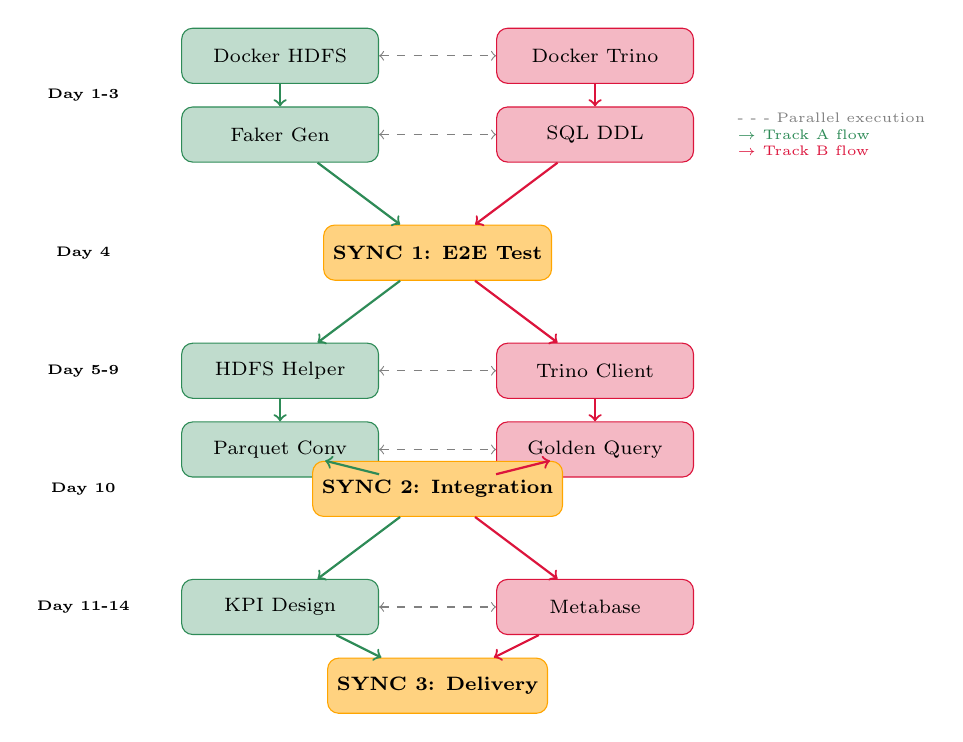
\begin{tikzpicture}[
    node distance=1.2cm,
    task/.style={rectangle, draw, rounded corners, minimum width=2.5cm, minimum height=0.7cm, font=\scriptsize},
    salmatask/.style={task, fill=salmacolor!30, draw=salmacolor},
    mohamedtask/.style={task, fill=mohamedcolor!30, draw=mohamedcolor},
    synctask/.style={task, fill=sharedcolor!50, draw=sharedcolor, font=\scriptsize\bfseries},
    arrow/.style={->, thick}
]

% Day labels
\node[font=\tiny\bfseries] at (-4.5, 0.5) {Day 1-3};
\node[font=\tiny\bfseries] at (-4.5, -1.5) {Day 4};
\node[font=\tiny\bfseries] at (-4.5, -3) {Day 5-9};
\node[font=\tiny\bfseries] at (-4.5, -4.5) {Day 10};
\node[font=\tiny\bfseries] at (-4.5, -6) {Day 11-14};

% Track A - Salma (Left side)
\node[salmatask] (s1) at (-2, 1) {Docker HDFS};
\node[salmatask] (s2) at (-2, 0) {Faker Gen};
\node[salmatask] (s3) at (-2, -3) {HDFS Helper};
\node[salmatask] (s4) at (-2, -4) {Parquet Conv};
\node[salmatask] (s5) at (-2, -6) {KPI Design};

% Track B - Mohamed (Right side)
\node[mohamedtask] (m1) at (2, 1) {Docker Trino};
\node[mohamedtask] (m2) at (2, 0) {SQL DDL};
\node[mohamedtask] (m3) at (2, -3) {Trino Client};
\node[mohamedtask] (m4) at (2, -4) {Golden Query};
\node[mohamedtask] (m5) at (2, -6) {Metabase};

% Sync points (Center)
\node[synctask] (sync1) at (0, -1.5) {SYNC 1: E2E Test};
\node[synctask] (sync2) at (0, -4.5) {SYNC 2: Integration};
\node[synctask] (sync3) at (0, -7) {SYNC 3: Delivery};

% Track A arrows (independent flow)
\draw[arrow, salmacolor] (s1) -- (s2);
\draw[arrow, salmacolor] (s2) -- (sync1);
\draw[arrow, salmacolor] (sync1) -- (s3);
\draw[arrow, salmacolor] (s3) -- (s4);
\draw[arrow, salmacolor] (s4) -- (sync2);
\draw[arrow, salmacolor] (sync2) -- (s5);
\draw[arrow, salmacolor] (s5) -- (sync3);

% Track B arrows (independent flow)
\draw[arrow, mohamedcolor] (m1) -- (m2);
\draw[arrow, mohamedcolor] (m2) -- (sync1);
\draw[arrow, mohamedcolor] (sync1) -- (m3);
\draw[arrow, mohamedcolor] (m3) -- (m4);
\draw[arrow, mohamedcolor] (m4) -- (sync2);
\draw[arrow, mohamedcolor] (sync2) -- (m5);
\draw[arrow, mohamedcolor] (m5) -- (sync3);

% Parallel indicators
\draw[<->, dashed, gray] (s1) -- (m1);
\draw[<->, dashed, gray] (s2) -- (m2);
\draw[<->, dashed, gray] (s3) -- (m3);
\draw[<->, dashed, gray] (s4) -- (m4);
\draw[<->, dashed, gray] (s5) -- (m5);

% Legend
\node[font=\tiny, align=left] at (5, 0) {
    \textcolor{gray}{- - - Parallel execution}\\
    \textcolor{salmacolor}{$\rightarrow$ Track A flow}\\
    \textcolor{mohamedcolor}{$\rightarrow$ Track B flow}
};

\end{tikzpicture}
\end{center}

\textbf{Critical Path:} Both tracks have equal length (14 days). Neither person blocks the other.

\begin{table}[h!]
\centering
\scriptsize
\begin{tabular}{|p{3cm}|c|c|p{5cm}|}
\hline
\rowcolor{primaryblue!20}
\textbf{Dependency Type} & \textbf{Count} & \textbf{Impact} & \textbf{Resolution} \\
\hline
Blocking (A waits for B) & 0 & None & No blocking dependencies \\
\hline
Blocking (B waits for A) & 0 & None & No blocking dependencies \\
\hline
Sync Required & 3 & Low & Days 4, 10, 14 only \\
\hline
Shared Resource & 1 & Low & docker-compose.yml (split sections) \\
\hline
Data Handoff & 1 & Low & Day 4: Faker IDs $\rightarrow$ SQL validation \\
\hline
\end{tabular}
\caption{Dependency Analysis Summary}
\end{table}

\begin{table}[h!]
\centering
\begin{tabular}{|l|l|}
\hline
\cellcolor{salmacolor!50} S: & SAID Salma Tasks \\
\hline
\cellcolor{mohamedcolor!50} M: & TAMZIRT Mohamed Tasks \\
\hline
\cellcolor{sharedcolor!50} BOTH: & Shared/Collaboration Tasks \\
\hline
\end{tabular}
\caption{Legend}
\end{table}

\newpage

% ============================================
% SECTION 6: FILE RESPONSIBILITY MATRIX
% ============================================
\section{File Responsibility Matrix}

\subsection{Ownership by File}

\begin{longtable}{|p{5.5cm}|c|c|c|p{2cm}|}
\hline
\rowcolor{primaryblue!30}
\textbf{File Path} & \textbf{Salma} & \textbf{Mohamed} & \textbf{Shared} & \textbf{Complexity} \\
\hline
\endhead

\multicolumn{5}{|l|}{\cellcolor{gray!20}\textbf{Docker Configuration (Split Ownership)}} \\
\hline
docker/docker-compose.yml & \checkmark & \checkmark & & HIGH \\
\hline
docker/hadoop-conf/core-site.xml & \checkmark & & & MEDIUM \\
\hline
docker/hadoop-conf/hdfs-site.xml & \checkmark & & & MEDIUM \\
\hline
docker/trino-conf/config.properties & & \checkmark & & HIGH \\
\hline
docker/trino-conf/catalog/hive.properties & & \checkmark & & HIGH \\
\hline
docker/trino-conf/catalog/postgres.properties & & \checkmark & & MEDIUM \\
\hline

\multicolumn{5}{|l|}{\cellcolor{gray!20}\textbf{Airflow DAGs \& Utilities}} \\
\hline
dags/procurement\_dag.py & & \checkmark & & HIGH \\
\hline
dags/utils/hdfs\_helper.py & \checkmark & & & HIGH \\
\hline
dags/utils/trino\_client.py & & \checkmark & & HIGH \\
\hline

\multicolumn{5}{|l|}{\cellcolor{gray!20}\textbf{Source Code - Data Generation}} \\
\hline
src/generator/main.py & \checkmark & & & HIGH \\
\hline
src/generator/entities.py & \checkmark & & & MEDIUM \\
\hline

\multicolumn{5}{|l|}{\cellcolor{gray!20}\textbf{Source Code - SQL}} \\
\hline
src/sql/ddl\_postgres.sql & & \checkmark & & HIGH \\
\hline
src/sql/ddl\_hive.sql & & \checkmark & & MEDIUM \\
\hline
src/sql/net\_demand.sql & & \checkmark & & CRITICAL \\
\hline
src/sql/parquet\_opt.sql & & \checkmark & & MEDIUM \\
\hline

\multicolumn{5}{|l|}{\cellcolor{gray!20}\textbf{Analytics}} \\
\hline
src/analytics/dashboard\_setup.sql & \checkmark & \checkmark & & HIGH \\
\hline

\multicolumn{5}{|l|}{\cellcolor{gray!20}\textbf{Data Directories}} \\
\hline
data/raw/* & \checkmark & & & -- \\
\hline
data/output/* & & & \checkmark & -- \\
\hline

\multicolumn{5}{|l|}{\cellcolor{gray!20}\textbf{Documentation}} \\
\hline
README.md (Setup Section) & \checkmark & & & MEDIUM \\
\hline
README.md (Usage Section) & & \checkmark & & MEDIUM \\
\hline
requirements.txt & & & \checkmark & LOW \\
\hline

\caption{File Ownership and Complexity Matrix}
\end{longtable}

\subsection{Complexity Summary by Owner}

\begin{table}[h!]
\centering
\begin{tabular}{|l|c|c|c|c|c|}
\hline
\rowcolor{primaryblue!30}
\textbf{Owner} & \textbf{CRITICAL} & \textbf{HIGH} & \textbf{MEDIUM} & \textbf{LOW} & \textbf{Total Files} \\
\hline
\cellcolor{salmacolor!20}SAID Salma & 0 & 4 & 4 & 0 & 8 \\
\hline
\cellcolor{mohamedcolor!20}TAMZIRT Mohamed & 1 & 5 & 3 & 0 & 9 \\
\hline
\cellcolor{sharedcolor!20}Shared & 0 & 1 & 0 & 1 & 2 \\
\hline
\end{tabular}
\caption{Complexity Distribution - Balanced Workload}
\end{table}

\newpage

% ============================================
% SECTION 7: SYNCHRONIZATION POINTS
% ============================================
\section{Synchronization Points}

\begin{sharedbox}[Critical Coordination Meetings]
Both team members must synchronize at these critical points to ensure integration success. \textbf{Evening syncs} are brief 15-minute check-ins. \textbf{Full syncs} are 1-2 hour working sessions.
\end{sharedbox}

\subsection{Daily Evening Syncs (15 min)}

\begin{table}[h!]
\centering
\scriptsize
\begin{tabular}{|c|p{5cm}|p{5cm}|p{3cm}|}
\hline
\rowcolor{primaryblue!20}
\textbf{Day} & \cellcolor{salmacolor!20}\textbf{Salma Reports} & \cellcolor{mohamedcolor!20}\textbf{Mohamed Reports} & \textbf{Decision Point} \\
\hline
1 & HDFS/Airflow containers status & Trino/Postgres containers status & Network connectivity \\
\hline
3 & Faker data structure ready & PostgreSQL sample data IDs & \textbf{ID Mapping Sync} \\
\hline
6 & HDFS helper methods complete & DAG task structure ready & Integration approach \\
\hline
8 & Parquet conversion working & Golden Query tested & Performance review \\
\hline
11 & Dashboard designs prepared & Metabase connection ready & KPI prioritization \\
\hline
13 & Infrastructure docs complete & SQL/DAG docs complete & README merge plan \\
\hline
\end{tabular}
\caption{Evening Sync Schedule}
\end{table}

\subsection{Sync Point 1: Day 4 - Manual End-to-End Validation}

\begin{table}[h!]
\centering
\begin{tabular}{|p{3cm}|p{10cm}|}
\hline
\rowcolor{primaryblue!20}
\textbf{Aspect} & \textbf{Details} \\
\hline
\textbf{Duration} & 2 hours (Full Working Session) \\
\hline
\textbf{Purpose} & Validate end-to-end data flow before automation phase \\
\hline
\cellcolor{salmacolor!20}\textbf{Salma's Input} & \begin{itemize}[nosep,leftmargin=*]
    \item Test Parquet files (orders + inventory)
    \item HDFS directories created (/raw/orders, /raw/stock)
    \item Sample data uploaded to HDFS
\end{itemize} \\
\hline
\cellcolor{mohamedcolor!20}\textbf{Mohamed's Input} & \begin{itemize}[nosep,leftmargin=*]
    \item PostgreSQL master data loaded
    \item Hive external tables created
    \item Federated query prepared
\end{itemize} \\
\hline
\textbf{Joint Activities} & \begin{enumerate}[nosep,leftmargin=*]
    \item Execute federated query in Trino CLI
    \item Verify JOIN results are non-empty
    \item Validate Product ID mappings
    \item Document any schema adjustments needed
\end{enumerate} \\
\hline
\textbf{Success Criteria} & Query returns $\geq$ 5 rows with correct supplier-product joins \\
\hline
\textbf{Fallback} & Re-check Product ID mappings; regenerate Faker data if needed \\
\hline
\end{tabular}
\caption{Day 4 Sync - Manual Validation Details}
\end{table}

\subsection{Sync Point 2: Day 10 - Full Pipeline Integration Test}

\begin{table}[h!]
\centering
\begin{tabular}{|p{3cm}|p{10cm}|}
\hline
\rowcolor{primaryblue!20}
\textbf{Aspect} & \textbf{Details} \\
\hline
\textbf{Duration} & 3 hours (Full Working Session) \\
\hline
\textbf{Purpose} & Complete pipeline automation test \\
\hline
\cellcolor{salmacolor!20}\textbf{Salma's Input} & \begin{itemize}[nosep,leftmargin=*]
    \item HDFS helper module fully tested
    \item Batch ingestion function working
    \item Idempotent purging verified
    \item Parquet conversion operational
\end{itemize} \\
\hline
\cellcolor{mohamedcolor!20}\textbf{Mohamed's Input} & \begin{itemize}[nosep,leftmargin=*]
    \item Airflow DAG with all 3 tasks
    \item Trino client module tested
    \item Golden Query optimized
    \item JSON export function ready
\end{itemize} \\
\hline
\textbf{Joint Activities} & \begin{enumerate}[nosep,leftmargin=*]
    \item Trigger manual DAG run in Airflow UI
    \item Monitor task execution in real-time
    \item Verify HDFS data ingestion
    \item Check Net Demand calculation results
    \item Validate JSON output file
    \item Test idempotency (re-run for same date)
\end{enumerate} \\
\hline
\textbf{Success Criteria} & \begin{itemize}[nosep,leftmargin=*]
    \item All 3 DAG tasks complete successfully
    \item JSON file generated in data/output/
    \item Re-run produces identical results (idempotent)
\end{itemize} \\
\hline
\textbf{Fallback} & Debug failing task; check XCom data passing \\
\hline
\end{tabular}
\caption{Day 10 Sync - Integration Test Details}
\end{table}

\subsection{Sync Point 3: Day 14 - Final Delivery \& Presentation}

\begin{table}[h!]
\centering
\begin{tabular}{|p{3cm}|p{10cm}|}
\hline
\rowcolor{primaryblue!20}
\textbf{Aspect} & \textbf{Details} \\
\hline
\textbf{Duration} & 4 hours (Final Review + Presentation Prep) \\
\hline
\textbf{Purpose} & Project completion, documentation merge, presentation \\
\hline
\textbf{Deliverables} & \begin{itemize}[nosep,leftmargin=*]
    \item Complete working pipeline
    \item Metabase dashboards with 3 KPIs
    \item Merged README.md
    \item Project report
\end{itemize} \\
\hline
\textbf{Joint Activities} & \begin{enumerate}[nosep,leftmargin=*]
    \item Merge documentation sections
    \item Final pipeline demonstration
    \item Dashboard walkthrough
    \item Prepare presentation slides
    \item Clean up test artifacts
\end{enumerate} \\
\hline
\textbf{Presentation Split} & \begin{itemize}[nosep,leftmargin=*]
    \item \textbf{Salma:} Infrastructure, HDFS, Data Generation
    \item \textbf{Mohamed:} Trino, SQL, DAG, Metabase
\end{itemize} \\
\hline
\end{tabular}
\caption{Day 14 Sync - Final Delivery Details}
\end{table}

\newpage

% ============================================
% SECTION 8: RISK MANAGEMENT
% ============================================
\section{Risk Management by Owner}

\begin{table}[h!]
\centering
\small
\begin{tabular}{|p{2.5cm}|p{1.5cm}|p{2cm}|p{6.5cm}|}
\hline
\rowcolor{primaryblue!30}
\textbf{Risk} & \textbf{Impact} & \textbf{Owner} & \textbf{Mitigation Strategy} \\
\hline
RAM Scarcity & High & \cellcolor{salmacolor!20}Salma & Disable Metabase until Day 11; apply memory limits in Docker Compose; monitor with \texttt{docker stats} \\
\hline
ID Mismatch & Critical & \cellcolor{sharedcolor!20}Both & Cross-validate on Day 3 evening sync; use constants file shared between Faker and DDL \\
\hline
Trino Connectivity & High & \cellcolor{mohamedcolor!20}Mohamed & Ensure Hive Metastore is initialized by Day 2; test catalog connections individually \\
\hline
HDFS Write Failures & Medium & \cellcolor{salmacolor!20}Salma & Test HDFS permissions on Day 1; verify safe mode is off; check datanode health \\
\hline
DAG Task Failures & Medium & \cellcolor{mohamedcolor!20}Mohamed & Implement retry logic (2 retries); add proper error handling and logging \\
\hline
Parquet Schema Issues & Medium & \cellcolor{salmacolor!20}Salma & Validate schema before upload; use PyArrow schema enforcement \\
\hline
Query Performance & Medium & \cellcolor{mohamedcolor!20}Mohamed & Add indexes in PostgreSQL; optimize JOIN order; test with increasing data volumes \\
\hline
Network Issues & Low & \cellcolor{sharedcolor!20}Both & Use Docker internal network; avoid port conflicts; document all exposed ports \\
\hline
\end{tabular}
\caption{Risk Management Matrix with Ownership}
\end{table}

\section{Quality Assurance Checklist}

\subsection{Phase 1 Quality Gates (Day 4)}

\begin{table}[h!]
\centering
\begin{tabular}{|p{6cm}|c|c|c|}
\hline
\rowcolor{primaryblue!20}
\textbf{Quality Check} & \cellcolor{salmacolor!20}\textbf{Salma} & \cellcolor{mohamedcolor!20}\textbf{Mohamed} & \textbf{Status} \\
\hline
All 11 Docker containers running & \checkmark & \checkmark & $\square$ \\
\hline
HDFS directories created & \checkmark & & $\square$ \\
\hline
Trino catalogs responding & & \checkmark & $\square$ \\
\hline
PostgreSQL master data loaded & & \checkmark & $\square$ \\
\hline
Faker generates valid data & \checkmark & & $\square$ \\
\hline
Federated query returns results & \checkmark & \checkmark & $\square$ \\
\hline
\end{tabular}
\caption{Phase 1 Quality Checklist}
\end{table}

\subsection{Phase 2 Quality Gates (Day 10)}

\begin{table}[h!]
\centering
\begin{tabular}{|p{6cm}|c|c|c|}
\hline
\rowcolor{primaryblue!20}
\textbf{Quality Check} & \cellcolor{salmacolor!20}\textbf{Salma} & \cellcolor{mohamedcolor!20}\textbf{Mohamed} & \textbf{Status} \\
\hline
HDFS helper all methods tested & \checkmark & & $\square$ \\
\hline
Trino client all methods tested & & \checkmark & $\square$ \\
\hline
DAG runs without errors & & \checkmark & $\square$ \\
\hline
Batch ingestion idempotent & \checkmark & & $\square$ \\
\hline
Golden Query returns correct results & & \checkmark & $\square$ \\
\hline
JSON export formatted correctly & & \checkmark & $\square$ \\
\hline
Parquet conversion working & \checkmark & & $\square$ \\
\hline
End-to-end pipeline successful & \checkmark & \checkmark & $\square$ \\
\hline
\end{tabular}
\caption{Phase 2 Quality Checklist}
\end{table}

\subsection{Phase 3 Quality Gates (Day 14)}

\begin{table}[h!]
\centering
\begin{tabular}{|p{6cm}|c|c|c|}
\hline
\rowcolor{primaryblue!20}
\textbf{Quality Check} & \cellcolor{salmacolor!20}\textbf{Salma} & \cellcolor{mohamedcolor!20}\textbf{Mohamed} & \textbf{Status} \\
\hline
Metabase connected to Trino & & \checkmark & $\square$ \\
\hline
3 KPI dashboards created & \checkmark & \checkmark & $\square$ \\
\hline
Documentation complete & \checkmark & \checkmark & $\square$ \\
\hline
README.md merged and reviewed & \checkmark & \checkmark & $\square$ \\
\hline
Code commented and clean & \checkmark & \checkmark & $\square$ \\
\hline
Presentation slides ready & \checkmark & \checkmark & $\square$ \\
\hline
\end{tabular}
\caption{Phase 3 Quality Checklist}
\end{table}

% ============================================
% SECTION 9: APPENDIX
% ============================================
\section{Appendix: Quick Reference Commands}

\subsection{For SAID Salma - Infrastructure \& Data}

\begin{lstlisting}[language=bash, caption={Docker \& HDFS Commands}]
# =====================================================
# DOCKER COMMANDS
# =====================================================
# Start Docker Stack (Full)
cd docker && docker-compose up -d

# Start without Metabase (Days 1-10 for RAM saving)
cd docker && docker-compose up -d --scale metabase=0

# Check container status
docker ps --format "table {{.Names}}\t{{.Status}}\t{{.Ports}}"

# View container logs
docker logs -f namenode
docker logs -f airflow-webserver

# Monitor RAM usage
docker stats --no-stream

# =====================================================
# HDFS COMMANDS
# =====================================================
# Check HDFS Health
docker exec -it namenode hdfs dfsadmin -report

# Leave Safe Mode (if stuck)
docker exec -it namenode hdfs dfsadmin -safemode leave

# Create HDFS Directories
docker exec -it namenode hdfs dfs -mkdir -p /raw/orders
docker exec -it namenode hdfs dfs -mkdir -p /raw/stock
docker exec -it namenode hdfs dfs -mkdir -p /processed

# Upload Test Data
docker exec -it namenode hdfs dfs -put /data/test.parquet /raw/orders/

# Check Directory Contents
docker exec -it namenode hdfs dfs -ls -R /raw/

# Check File Size
docker exec -it namenode hdfs dfs -du -h /raw/

# Remove Directory (for idempotency testing)
docker exec -it namenode hdfs dfs -rm -r /raw/orders/2025-12-29

# =====================================================
# PYTHON DATA GENERATION
# =====================================================
# Run Faker script
python src/generator/main.py --date 2025-12-29 --orders 100

# Validate Parquet file
python -c "import pyarrow.parquet as pq; print(pq.read_table('data/raw/orders.parquet').schema)"
\end{lstlisting}

\subsection{For TAMZIRT Mohamed - SQL \& Orchestration}

\begin{lstlisting}[language=bash, caption={Trino, PostgreSQL \& Airflow Commands}]
# =====================================================
# TRINO COMMANDS
# =====================================================
# Connect to Trino CLI
docker exec -it trino trino

# Test PostgreSQL Connection
trino> SHOW CATALOGS;
trino> SHOW SCHEMAS FROM postgres;
trino> SELECT * FROM postgres.master_data.products LIMIT 5;

# Test Hive Connection
trino> SHOW SCHEMAS FROM hive;
trino> SELECT * FROM hive.procurement_raw.orders LIMIT 5;

# Execute Federated Query Test
trino> SELECT p.product_name, o.quantity 
       FROM postgres.master_data.products p
       JOIN hive.procurement_raw.orders o 
       ON p.product_id = o.product_id
       LIMIT 10;

# Check Query Performance
trino> EXPLAIN ANALYZE SELECT ...;

# =====================================================
# POSTGRESQL COMMANDS
# =====================================================
# Connect to PostgreSQL
docker exec -it postgres psql -U admin -d procurement

# Execute DDL
psql> \i /sql/ddl_postgres.sql

# Check tables
psql> \dt master_data.*

# Verify data
psql> SELECT COUNT(*) FROM master_data.products;

# =====================================================
# HIVE METASTORE COMMANDS
# =====================================================
# Initialize Metastore Schema
docker exec -it hive-metastore schematool -dbType postgres -initSchema

# Execute Hive DDL
docker exec -it hive-metastore hive -f /sql/ddl_hive.sql

# Repair partitions after data load
docker exec -it hive-metastore hive -e "MSCK REPAIR TABLE procurement_raw.orders"

# =====================================================
# AIRFLOW COMMANDS
# =====================================================
# Access Airflow Web UI
# URL: http://localhost:8081 (user: airflow, pass: airflow)

# Trigger DAG manually
docker exec -it airflow-webserver airflow dags trigger procurement_pipeline

# Check DAG status
docker exec -it airflow-webserver airflow dags list

# View task logs
docker exec -it airflow-webserver airflow tasks logs procurement_pipeline calculate_net_demand 2025-12-29

# Test single task
docker exec -it airflow-webserver airflow tasks test procurement_pipeline batch_ingest_hdfs 2025-12-29
\end{lstlisting}

\subsection{Shared Commands - Both Team Members}

\begin{lstlisting}[language=bash, caption={Shared Utility Commands}]
# =====================================================
# GIT COMMANDS (for collaboration)
# =====================================================
# Pull latest changes before starting work
git pull origin main

# Create feature branch
git checkout -b feature/salma-hdfs-helper
git checkout -b feature/mohamed-trino-client

# Commit and push
git add .
git commit -m "[Salma] Add HDFS helper module"
git push origin feature/salma-hdfs-helper

# Merge to main (after review)
git checkout main
git merge feature/salma-hdfs-helper

# =====================================================
# TESTING COMMANDS
# =====================================================
# Run Python tests
pytest tests/ -v

# Validate SQL syntax
docker exec -it trino trino --execute "EXPLAIN ${SQL_QUERY}"

# Check JSON output
python -m json.tool data/output/supplier_orders_2025-12-29.json

# =====================================================
# METABASE (Day 11+)
# =====================================================
# Enable Metabase
docker-compose --profile visualization up -d metabase

# Access Metabase UI
# URL: http://localhost:3000
\end{lstlisting}

% ============================================
% END OF DOCUMENT
% ============================================

\newpage
\section{Final Summary: Two-Track Parallel Execution}

\subsection{Track Overview}

\begin{center}
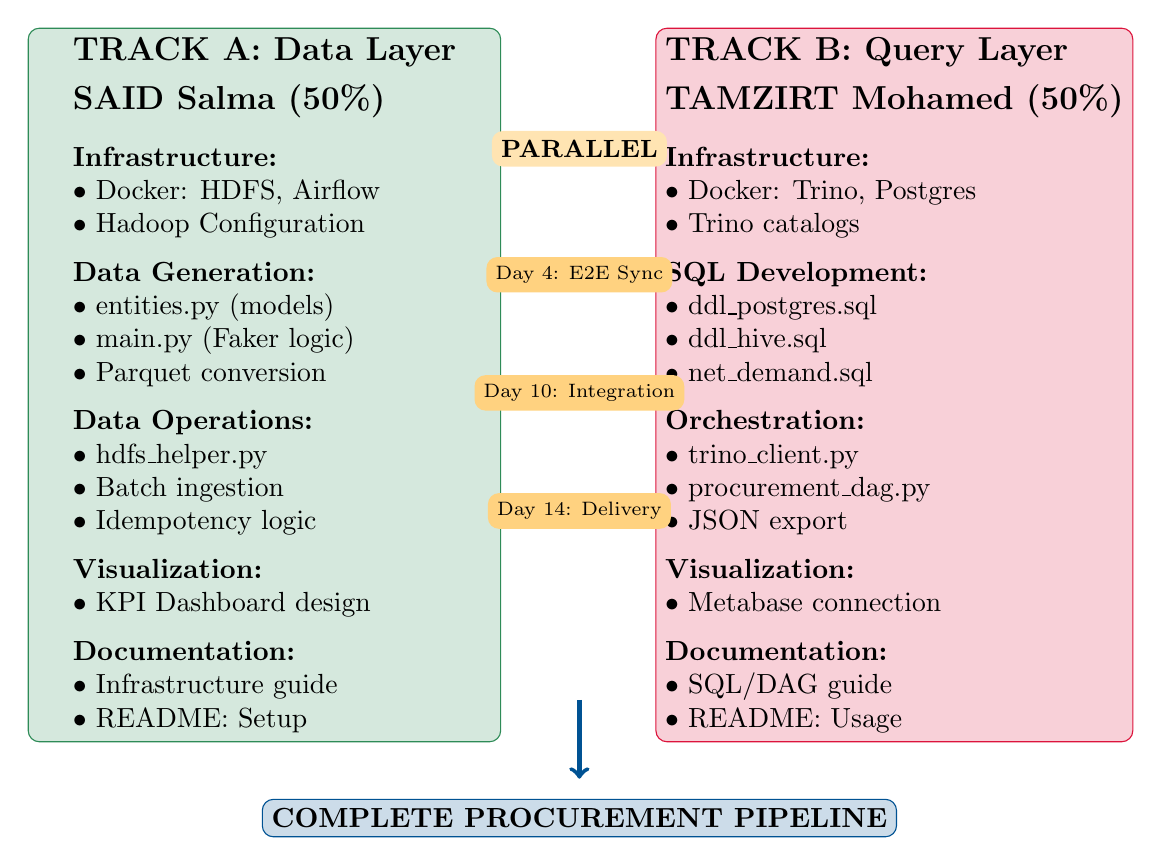
\begin{tikzpicture}
    % Track A - Salma
    \node[draw=salmacolor, fill=salmacolor!20, rounded corners, minimum width=6cm, minimum height=9cm, align=left] at (-4,0) {
        \textbf{\large TRACK A: Data Layer} \\[0.2cm]
        \textbf{\large SAID Salma (50\%)} \\[0.3cm]
        \textbf{Infrastructure:} \\
        $\bullet$ Docker: HDFS, Airflow \\
        $\bullet$ Hadoop Configuration \\[0.2cm]
        \textbf{Data Generation:} \\
        $\bullet$ entities.py (models) \\
        $\bullet$ main.py (Faker logic) \\
        $\bullet$ Parquet conversion \\[0.2cm]
        \textbf{Data Operations:} \\
        $\bullet$ hdfs\_helper.py \\
        $\bullet$ Batch ingestion \\
        $\bullet$ Idempotency logic \\[0.2cm]
        \textbf{Visualization:} \\
        $\bullet$ KPI Dashboard design \\[0.2cm]
        \textbf{Documentation:} \\
        $\bullet$ Infrastructure guide \\
        $\bullet$ README: Setup
    };
    
    % Track B - Mohamed
    \node[draw=mohamedcolor, fill=mohamedcolor!20, rounded corners, minimum width=6cm, minimum height=9cm, align=left] at (4,0) {
        \textbf{\large TRACK B: Query Layer} \\[0.2cm]
        \textbf{\large TAMZIRT Mohamed (50\%)} \\[0.3cm]
        \textbf{Infrastructure:} \\
        $\bullet$ Docker: Trino, Postgres \\
        $\bullet$ Trino catalogs \\[0.2cm]
        \textbf{SQL Development:} \\
        $\bullet$ ddl\_postgres.sql \\
        $\bullet$ ddl\_hive.sql \\
        $\bullet$ net\_demand.sql \\[0.2cm]
        \textbf{Orchestration:} \\
        $\bullet$ trino\_client.py \\
        $\bullet$ procurement\_dag.py \\
        $\bullet$ JSON export \\[0.2cm]
        \textbf{Visualization:} \\
        $\bullet$ Metabase connection \\[0.2cm]
        \textbf{Documentation:} \\
        $\bullet$ SQL/DAG guide \\
        $\bullet$ README: Usage
    };
    
    % Parallel indicator
    \draw[<->, ultra thick, sharedcolor] (-0.8,3) -- (0.8,3);
    \node[fill=sharedcolor!30, rounded corners, font=\small\bfseries] at (0,3) {PARALLEL};
    
    % Sync points with arrows
    \draw[->, thick, sharedcolor] (-0.8,1.5) -- (0.8,1.5);
    \draw[<-, thick, sharedcolor] (-0.8,1.3) -- (0.8,1.3);
    \node[fill=sharedcolor!50, rounded corners, font=\scriptsize] at (0,1.4) {Day 4: E2E Sync};
    
    \draw[->, thick, sharedcolor] (-0.8,0) -- (0.8,0);
    \draw[<-, thick, sharedcolor] (-0.8,-0.2) -- (0.8,-0.2);
    \node[fill=sharedcolor!50, rounded corners, font=\scriptsize] at (0,-0.1) {Day 10: Integration};
    
    \draw[->, thick, sharedcolor] (-0.8,-1.5) -- (0.8,-1.5);
    \draw[<-, thick, sharedcolor] (-0.8,-1.7) -- (0.8,-1.7);
    \node[fill=sharedcolor!50, rounded corners, font=\scriptsize] at (0,-1.6) {Day 14: Delivery};
    
    % Output arrow
    \draw[->, ultra thick, primaryblue] (0,-4) -- (0,-5);
    \node[draw=primaryblue, fill=primaryblue!20, rounded corners, minimum width=8cm, font=\bfseries] at (0,-5.5) {COMPLETE PROCUREMENT PIPELINE};
\end{tikzpicture}
\end{center}

\subsection{Workload Balance Verification}

\begin{table}[h!]
\centering
\begin{tabular}{|l|c|c|c|}
\hline
\rowcolor{primaryblue!30}
\textbf{Metric} & \cellcolor{salmacolor!30}\textbf{Person A (Salma)} & \cellcolor{mohamedcolor!30}\textbf{Person B (Mohamed)} & \textbf{Balance} \\
\hline
Total Hours & 54 & 54 & \textcolor{salmacolor}{\checkmark} 50/50 \\
\hline
HIGH Complexity Tasks & 4 & 5 & $\approx$ Equal \\
\hline
Python Files & 3 & 2 & $\approx$ Equal \\
\hline
SQL Files & 0 & 4 & Specialized \\
\hline
Config Files & 3 & 4 & $\approx$ Equal \\
\hline
Documentation Pages & 3 & 3 & \textcolor{salmacolor}{\checkmark} Equal \\
\hline
Sync Participation & 3 & 3 & \textcolor{salmacolor}{\checkmark} Equal \\
\hline
\end{tabular}
\caption{Workload Balance Verification}
\end{table}

\begin{tcolorbox}[colback=green!5, colframe=salmacolor, title=\textbf{Parallel Execution Guarantee}]
\textbf{This task distribution ensures:}
\begin{enumerate}
    \item \textbf{Zero blocking dependencies} between Person A and Person B
    \item \textbf{Natural specialization} - Data Layer vs Query Layer
    \item \textbf{50/50 effort split} - 54 hours each
    \item \textbf{Clear deliverables} - Each person owns specific files
    \item \textbf{Integration points} - Only 3 sync days required (Days 4, 10, 14)
\end{enumerate}
\end{tcolorbox}

\vfill
\begin{center}
\textcolor{primaryblue}{\rule{0.8\textwidth}{0.5pt}}

\textit{Document prepared for the Procurement Data Pipeline Project}

\textbf{Team: SAID Salma \& TAMZIRT Mohamed}

\textbf{Data Engineering Department - December 2025}

\vspace{0.5cm}
\textcolor{gray}{\small Equal contribution guaranteed through balanced task distribution and regular synchronization.}
\end{center}

\end{document}
